\documentclass{article} % For LaTeX2e
\usepackage{iclr2024_conference,times}

% Optional math commands from https://github.com/goodfeli/dlbook_notation.
\input{math_commands.tex}

\usepackage{booktabs}
\usepackage{hyperref}
\usepackage{url}
\usepackage{graphicx}
\usepackage{multirow}
\usepackage{xcolor}
\usepackage{enumitem}
\usepackage{float}
\renewcommand{\ttdefault}{cmtt} % Use CM Typewriter (available) instead of Courier (missing)

\iclrfinalcopy

\title{Study Coach: R2. Baseline and Proposal}

\author{
  Dipti Aswath \hspace{2em} Buddhika Makehelwala \hspace{2em} Jiashan Cui \hspace{2em} Khubi Shah \\
  \texttt{\{daswath, bmakehelwala, jiashanc, khubis\}@andrew.cmu.edu}
  }

\date{}

\begin{document}
\maketitle


\section{Baseline Models and Metrics (2 pages)}

We address \textbf{incongruence detection}: detecting mismatches between student explanations and scientific figures. Starting from SPIQA Test-A~\cite{pramanick2024spiqa}-a manually curated split of 666 QA pairs across 118 papers-we constructed \textbf{SPIQA+}, an augmented evaluation dataset, via a three-phase pipeline:
\begin{enumerate}[itemsep=6pt]
    \item \textbf{Prepare:} Filter SPIQA Test-A to figure-grounded QAs and annotate figure types (table, plot, figure/schematic).

    \item \textbf{Generate:} Hand-curate 18 In-Context Learning (ICL) exemplars covering all combinations: 3 figure types $\times$ 3 error categories (factual, conceptual, omission) $\times$ 2 verdicts (incorrect, partially correct). Use GPT-5.1 to synthetically generate incorrect and partially correct student answers with structured model responses.

    \item \textbf{Validate:} Human spot-check (${\sim}$20 examples), analyze error distribution, and enforce a quality gate ($\geq$90\% agreement).
\end{enumerate}
Each generated example follows a standardized \textbf{4-tuple} format: (1)~\textit{Context}-visual + textual context from the original SPIQA paper (figure + caption); (2)~\textit{Question}-the figure-grounded question from SPIQA; (3)~\textit{User Answer}-a synthetically generated student explanation (correct, partially correct, or incorrect); and (4)~\textit{Model Response}-a structured ground-truth containing a verdict, error category, and free-text coaching feedback (2--4 sentences). The resulting SPIQA+ dataset contains \textbf{174 generated examples} with the following distributions: error types are 48\% factual, 38\% conceptual, and 14\% omission; figure types are 70 tables, 68 plots, 32 schematics, and 4 other.

\textbf{Task setup.} Given a question about a scientific figure and a student's answer - which may be correct, partially correct, or incorrect - the model must:
\begin{enumerate}[itemsep=4pt]
    \item \textit{Detect mismatch} - classify the student's answer as correct, partially correct, or incorrect.\\
    \textcolor{gray}{\small``Is this explanation right?''}

    \item \textit{Categorize the error type} - identify whether the mistake is factual, conceptual, or an omission.\\
    \textcolor{gray}{\small``What kind of mistake?''}

    \item \textit{Provide coaching feedback} - localize and explain the error with constructive guidance.\\
    \textcolor{gray}{\small``Here's what you missed...''}
\end{enumerate}

This task is fundamentally multimodal: verifying ``BERT achieves 89\%'' requires reading the actual bar height (84.6\%) from the figure (visual grounding), while detecting a wrong conclusion requires mapping textual interpretations onto visual patterns (cross-modal reasoning).

The SPIQA paper established that paper context improves figure QA performance (Gemini 1.5 Pro achieves 8+ point L3Score improvements with full context). However, SPIQA only addresses: \textit{Can models generate correct answers?} It does not address: \textit{Can models evaluate whether a human's explanation is correct?} This answer evaluation capability is essential for educational applications like interview coaching. Because our model is evaluating a student's answer rather than generating its own, it receives \textbf{no reference answer} - it must reason directly from the figure and context to judge correctness. Including reference answers in early experiments reduced modality differences and lowered alignment with human judgment, so we removed them.

\textbf{Experimental conditions.} We test four input conditions to ablate the contribution of each modality:
\begin{itemize}[itemsep=4pt]
    \item \textbf{C1 (Text-Only):} Question + student answer only.\\
    No figure, no caption.

    \item \textbf{C2 (Caption-Only):} C1 + figure caption.\\
    Textual description of the figure, but no image.

    \item \textbf{C3 (Vision-Only):} C1 + figure image.\\
    Raw visual input, but no caption.

    \item \textbf{C4 (Multimodal):} C1 + figure image + caption.\\
    Full context available to the model.
\end{itemize}

\textbf{Hypotheses.} We test four hypotheses across these conditions:
\begin{enumerate}[itemsep=4pt]
    \item \textbf{H1 (Multimodal Advantage):} Visual input improves performance over text-only.

    \item \textbf{H2 (Metric Alignment):} Verdict accuracy and feedback quality will be correlated.

    \item \textbf{H3 (Error Type):} Factual errors will be detected more reliably than conceptual errors, and visual context will help conceptual errors more.

    \item \textbf{H4 (Figure Type):} Tables will be easiest (structured, localized information) and schematics hardest (distributed spatial relationships).
\end{enumerate}

\subsection{Unimodal Baselines}

Our unimodal baselines use \textbf{Qwen3-VL-8B}~\cite{bai2023qwenvl} under conditions C1 and C2, which provide only textual information. The Qwen-VL architecture uses a Vision Transformer (ViT) visual encoder initialized from OpenCLIP~\cite{bai2023qwenvl}, with a position-aware cross-attention adapter that compresses visual features to a fixed-length sequence of 256 tokens, which is then fed to the LLM backbone. This architecture was trained via a three-stage pipeline: large-scale image-text pretraining, multi-task pretraining at higher resolution ($448{\times}448$), and supervised fine-tuning for instruction following.

\textbf{C1 (Text-Only)} provides only the question and student answer. The model must rely on pre-trained knowledge to judge whether a claim like ``BERT achieves 89\% accuracy'' sounds plausible. C1 achieves the \textit{highest} verdict accuracy at 8B (56\%), revealing that the model does \textbf{plausibility checking}-judging whether claims sound reasonable-rather than verifying claims against the figure.

\textbf{C2 (Caption-Only)} adds the figure caption without the image. At 8B, C2 underperforms C1 on verdict (48\% vs 56\%), suggesting that at small scale, the caption introduces noise rather than helping classification. However, C2 shows improved feedback quality (46\% soft match vs 40\% for C1).

\subsection{Simple Multimodal Baselines}

We extend to multimodal conditions using the same Qwen3-VL-8B model under C3 and C4, which add figure images:

\textbf{C3 (Vision-Only)} provides the figure image but no caption. At 8B, C3 achieves 50\% verdict accuracy and 48\% soft match-better than C2 on feedback but worse than C1 on verdict.

\textbf{C4 (Multimodal)} provides both figure image and caption, giving the model full context. At 8B, C4 achieves the worst verdict accuracy (48\%) but the best feedback quality: 6\% exact match and 56\% soft match. Human evaluation on $n{=}10$ per condition confirmed this pattern even more dramatically: C4 achieved 80\% human-evaluated match versus C1's 40\% ($+$40pp). This dissociation-\textit{the model classifies worse but explains better with images}-was the central surprising finding from our midterm evaluation.

\subsection{Competitive Approaches}

To test whether model scale resolves the verdict--feedback dissociation, we evaluate \textbf{Qwen3-VL-32B}~\cite{bai2023qwenvl} across all four conditions. For direct comparison with the 8B baseline, Table~\ref{tab:h1h2} reports $N{=}50$ per condition. Both models were also run on the full $N{=}174$ sample for error type (H3, Table~\ref{tab:h3}) and figure type (H4, Table~\ref{tab:h4}) analyses. We also evaluated LLaVA-1.5-7B~\cite{liu2023llava15} on the error type hypothesis; Qwen3-VL-32B outperformed it and was the only model where visual context improved conceptual verdict accuracy.

\begin{enumerate}[itemsep=6pt]
    \item \textbf{Qwen3-VL-32B (C4, Multimodal):} Our primary competitive approach. At 32B, C4 achieves 20\% exact feedback match - a $10{\times}$ improvement over C1's 2\% and a $3.3{\times}$ improvement over the 8B C4 result (6\%). The verdict gap narrows from $-$8pp (8B) to $-$2pp (32B), suggesting scaling enables the model to extract useful signal from visual input.

    \item \textbf{Qwen3-VL-32B (C2, Caption-Only):} Achieves the best verdict accuracy at 32B (58\%), demonstrating that at scale, textual figure descriptions provide the most reliable classification signal. The $+$10pp improvement over 8B C2 (48\%) is the largest single-condition gain from scaling.

    \item \textbf{Qwen3-VL-32B (C1, Text-Only):} Serves as the scaled text-only reference. C1 verdict accuracy is unchanged at 56\%, but feedback quality remains poor (2\% match) - confirming that text-only feedback does not improve with scale.
\end{enumerate}

\begin{table}[H]
\centering
\small
\caption{H1/H2: Verdict accuracy and feedback quality by condition ($N{=}50$ per condition). Verdict = three-class classification (correct/partially correct/incorrect). Match \% and Soft Match \% = LLM-as-Judge (Claude Sonnet 4, temp=0). Human Match = manual evaluation ($n{=}10$, 8B only). H1 is read vertically (C1 vs C4); H2 is read horizontally (verdict vs feedback).}
\label{tab:h1h2}
\begin{tabular}{@{}lrrrrrrrr@{}}
\toprule
 & \multicolumn{4}{c}{Qwen3-VL-8B} & \multicolumn{4}{c}{Qwen3-VL-32B} \\
\cmidrule(lr){2-5} \cmidrule(l){6-9}
Condition & Verdict & Match & Soft M. & Human & Verdict & Match & Soft M. & Human \\
\midrule
C1: Text-Only     & \textbf{56\%} & 2\%  & 40\% & 40\% & 56\%          & 2\%           & 42\% & - \\
C2: Caption-Only  & 48\%          & 2\%  & 46\% & 50\% & \textbf{58\%} & 8\%           & 48\% & - \\
C3: Vision-Only   & 50\%          & 4\%  & 48\% & 60\% & 56\%          & 6\%           & 48\% & - \\
C4: Multimodal    & 48\%          & 6\%  & 56\% & 80\% & 54\%          & \textbf{20\%} & \textbf{58\%} & - \\
\midrule
$\Delta$ (C4$-$C1) & $-$8pp & +4pp & +16pp & +40pp & $-$2pp & +18pp & +16pp & - \\
\bottomrule
\end{tabular}
\end{table}

\begin{table}[H]
\centering
\small
\caption{H3: Verdict accuracy and feedback match by error type ($N{=}174$; 52 factual, 41 conceptual, 15 omission). Avg = average across C1--C4. $\Delta$ = C4$-$C1, measuring the benefit of visual context.}
\label{tab:h3}
\begin{tabular}{@{}lrrrrrrrr@{}}
\toprule
 & \multicolumn{4}{c}{Qwen3-VL-8B} & \multicolumn{4}{c}{Qwen3-VL-32B} \\
\cmidrule(lr){2-5} \cmidrule(l){6-9}
Error Type & Verd. Avg & Verd. $\Delta$ & Fdbk Avg & Fdbk $\Delta$ & Verd. Avg & Verd. $\Delta$ & Fdbk Avg & Fdbk $\Delta$ \\
\midrule
Factual     & 39.4\% & $-$21.2pp & 25.5\% & +21.2pp & 28.4\% & $-$7.7pp          & 26.0\% & +21.2pp \\
Conceptual  & 54.3\% & $-$14.6pp & 43.3\% & +31.7pp & 57.3\% & \textbf{+2.4pp}   & 42.1\% & +29.3pp \\
Omission    & 45.0\% & $-$6.7pp  & 15.0\% & +33.3pp & 48.3\% & $-$26.7pp         & 13.4\% & +26.7pp \\
\bottomrule
\end{tabular}
\end{table}

\noindent\textbf{Reading Table~\ref{tab:h3}:} H3 predicted factual errors would be easiest (explicit visual grounding) and visual context would help conceptual errors most. Both predictions partially failed. \textit{Verdict accuracy:} Conceptual errors are consistently easier than factual (54.3\% vs 39.4\% at 8B; 57.3\% vs 28.4\% at 32B)---the model detects logical inconsistencies in text more reliably than it verifies specific numerical claims against the figure. The $+$2.4pp for 32B conceptual (bolded) represents the \textit{only} cell where visual context improves verdict accuracy: 25/41 correct with images vs 24/41 without. \textit{Feedback quality:} Visual context helps all error types at both scales ($+$21--33pp), with the largest gains for omission errors ($+$33.3pp at 8B) where seeing the figure reveals what the student failed to mention.

\begin{table}[H]
\centering
\small
\caption{H4: Verdict accuracy and feedback match by figure type ($N{=}174$; 70 tables, 68 plots, 32 schematics). Avg = average across C1--C4. $\Delta$ = C4$-$C1.}
\label{tab:h4}
\begin{tabular}{@{}lrrrrrrrr@{}}
\toprule
 & \multicolumn{4}{c}{Qwen3-VL-8B} & \multicolumn{4}{c}{Qwen3-VL-32B} \\
\cmidrule(lr){2-5} \cmidrule(l){6-9}
Figure Type & Verd. Avg & Verd. $\Delta$ & Fdbk Avg & Fdbk $\Delta$ & Verd. Avg & Verd. $\Delta$ & Fdbk Avg & Fdbk $\Delta$ \\
\midrule
Table       & 51.4\% & $-$2.9pp  & 6.4\%  & +7.1pp  & 51.1\% & +1.4pp           & 12.1\% & +15.7pp \\
Plot        & 47.8\% & $-$10.3pp & 21.7\% & +19.1pp & 49.3\% & $-$4.4pp         & 26.5\% & +33.8pp \\
Schematic   & 48.4\% & +9.4pp    & 35.2\% & +25.0pp & \textbf{57.0\%} & \textbf{+18.8pp} & \textbf{46.1\%} & +25.0pp \\
\bottomrule
\end{tabular}
\end{table}

\noindent\textbf{Reading Table~\ref{tab:h4}:} H4 predicted tables would be easiest (structured, localized data) and schematics hardest (spatial reasoning). Results are mixed. \textit{Verdict accuracy:} At 8B, tables are slightly easiest (51.4\% avg), but at 32B schematics overtake them (57.0\% vs 51.1\%, bolded). The $+$18.8pp schematic gain at 32B (bolded) shows visual context dramatically helps spatial reasoning at scale---the model leverages the figure to understand component relationships. Plots are consistently hurt by visual context ($-$10.3pp at 8B, $-$4.4pp at 32B), suggesting trend interpretation remains challenging. \textit{Feedback quality:} Schematics achieve the highest feedback match at both scales (35.2\% at 8B, 46.1\% at 32B, bolded), while tables are worst (6.4\% at 8B, 12.1\% at 32B)---structured data is easier to \textit{classify} but harder to \textit{explain}. Visual context helps feedback for all figure types ($+$7--34pp), with plots showing the largest 32B gain ($+$33.8pp).

\section{Results (1 page)}

Tables~\ref{tab:h1h2}--\ref{tab:h4} summarize results across all four hypotheses, both model scales, and four input conditions.

\paragraph{Metric 1: Verdict Accuracy (three-class classification).}
The model classifies student answers as correct, partially correct, or incorrect.

\begin{itemize}[itemsep=2pt, topsep=2pt]
    \item \textbf{H1} (Table~\ref{tab:h1h2}): Visual input \textit{hurts} verdict accuracy at both scales.
    \begin{itemize}[itemsep=1pt, topsep=1pt]
        \item 8B: C1 (text-only) wins at 56\%; C4 (multimodal) worst at 48\% ($\Delta{=}-$8pp)
        \item 32B: Gap narrows---C2 leads at 58\%, C4 reaches 54\% ($\Delta{=}-$2pp)
    \end{itemize}
    \item \textbf{H3} (Table~\ref{tab:h3}): Conceptual errors easier than factual (opposite of hypothesis).
    \begin{itemize}[itemsep=1pt, topsep=1pt]
        \item Factual: 39.4\% (8B), 28.4\% (32B)---hardest error type
        \item Conceptual: 54.3\% (8B), 57.3\% (32B)---easiest error type
        \item 32B conceptual is the \textit{only} cell where visual context helps verdict ($+$2.4pp)
    \end{itemize}
    \item \textbf{H4} (Table~\ref{tab:h4}): Schematics benefit most; plots hurt most.
    \begin{itemize}[itemsep=1pt, topsep=1pt]
        \item Schematics: $+$9.4pp (8B), $+$18.8pp (32B)---visual context helps
        \item Plots: $-$10.3pp (8B), $-$4.4pp (32B)---visual context hurts
    \end{itemize}
\end{itemize}

\paragraph{Metric 2: Feedback Match Rate (LLM-as-Judge).}
Since traditional auto metrics (F1, ROUGE-L, BLEU) fail to differentiate feedback quality across conditions (see Appendix, Table~\ref{tab:auto_metrics}), we use Claude Sonnet~4 as an automated judge. Each predicted feedback is classified into one of three categories:

\begin{itemize}[itemsep=1pt, topsep=2pt]
  \item \textbf{Match} --- the model's feedback aligns with the ground-truth explanation: it correctly identifies what is wrong and explains why.
  \item \textbf{Partial} --- the feedback captures some of the right reasoning but misses key elements, or gets the direction right but is imprecise.
  \item \textbf{Unmatched} --- the feedback does not align with the ground truth.
\end{itemize}

\noindent We report \textbf{Match\%} (strict: exact matches only) and \textbf{Soft Match\%} (Match + Partial). The gap between them is informative: at 32B, C4 achieves 20\% strict match but 58\% soft match---meaning 38\% of responses are approximately correct but not precise. Human evaluation ($n{=}10$/condition, 8B) confirmed the pattern: human match ranged from 40\% (C1) to 80\% (C4), tracking closer to soft match, validating it as the practical metric for coaching.

\begin{itemize}[itemsep=2pt, topsep=2pt]
    \item \textbf{H1}: Visual input \textit{helps} feedback quality dramatically.
    \begin{itemize}[itemsep=1pt, topsep=1pt]
        \item C4 at 32B: 20\% exact match ($10{\times}$ improvement over C1's 2\%)
        \item All error types benefit: $+$21--33pp (Table~\ref{tab:h3})
        \item All figure types benefit: $+$7--34pp (Table~\ref{tab:h4})
    \end{itemize}
    \item \textbf{H2}: Verdict and feedback are \textit{inversely correlated}.
    \begin{itemize}[itemsep=1pt, topsep=1pt]
        \item C1/C2 classify best but produce worst feedback
        \item C4 classifies worst but explains best
    \end{itemize}
\end{itemize}

\paragraph{Metric 3: Soft Match Rate (Match + Partial).}
Soft Match counts feedback that is at least partially useful for coaching---the practical metric for StudyCoach.

\begin{itemize}[itemsep=2pt, topsep=2pt]
    \item C4 at 32B: 58\% soft match vs 42\% for C1 ($+$16pp)
    \item Human evaluation confirms: 40\% (C1) $\to$ 80\% (C4) tracks soft match
\end{itemize}

\vspace{4pt}
\noindent\fbox{\parbox{0.97\linewidth}{\textbf{Key insight:} The verdict--feedback dissociation (H2) holds across all error types and figure types at both scales. \textit{StudyCoach should use condition routing: text-only for grading, multimodal for coaching.}}}

\vspace{6pt}
\noindent\textbf{Appendix Guide:} For detailed breakdowns supporting these results, see:
\begin{itemize}[itemsep=1pt, topsep=2pt, leftmargin=*]
  \item \textbf{Table~\ref{tab:hypotheses}} --- Summary of all hypothesis outcomes across metrics and scales
  \item \textbf{Tables~\ref{tab:h3_verdict}--\ref{tab:h3_feedback}} --- H3 condition-level breakdown (C1--C4) by error type
  \item \textbf{Tables~\ref{tab:h4_verdict}--\ref{tab:h4_feedback}} --- H4 condition-level breakdown (C1--C4) by figure type
  \item \textbf{Table~\ref{tab:auto_metrics}} --- Auto metrics comparison showing why LLM-as-Judge was necessary
\end{itemize}

\section{Model Proposal (1 Page)}

\subsection{\points{1.5} Overall Model Structure}

Our Study Coach system evaluates student answers to figure-grounded questions from scientific papers. We selected three vision-language models (VLMs) that share a common architecture: a \textbf{vision encoder} that converts figure images into patch-level features, a \textbf{cross-modal connector} that projects visual features into the language model's embedding space, and a \textbf{decoder-only LLM} that auto-regressively generates the verdict, error category, and coaching feedback.

The models differ in their approach to \textbf{transference}---transferring knowledge between modalities \citep{Liang-foundations-2024}. LLaVA-1.5 uses \emph{cross-modal transfer} from a frozen CLIP encoder, while Qwen3-VL uses \emph{co-learning} via joint encoder-decoder training. Our 8B baseline results show this distinction matters: text\_only verdict accuracy (56\%) outperformed multimodal (48\%), suggesting transferred visual representations can introduce noise at 8B scale---though they substantially improve explanation quality (80\% vs.\ 40\% human match rate).

\begin{figure}[H]
\centering
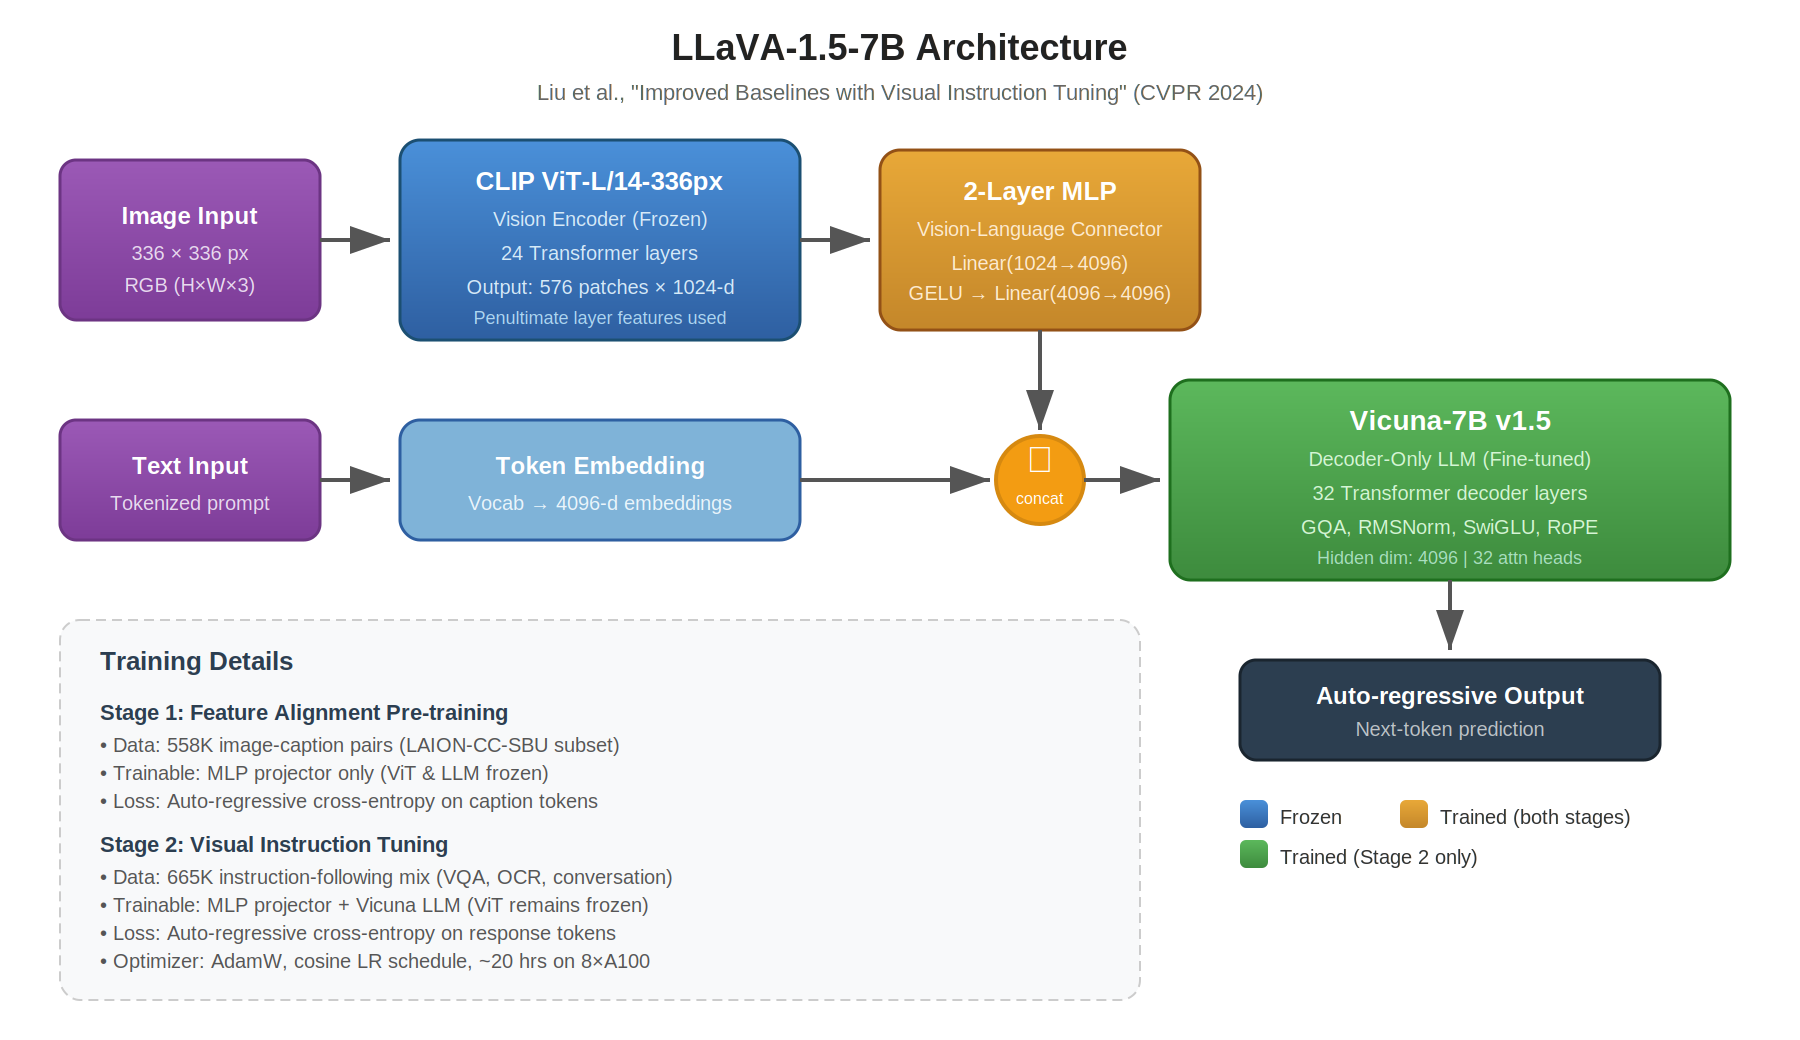
\includegraphics[width=0.95\textwidth]{figures/llava_architecture.png}
\caption{LLaVA-1.5-7B architecture: frozen CLIP ViT-L/14 $\rightarrow$ 2-layer MLP $\rightarrow$ Vicuna-7B.}
\label{fig:llava-arch}
\end{figure}

\begin{figure}[H]
\centering
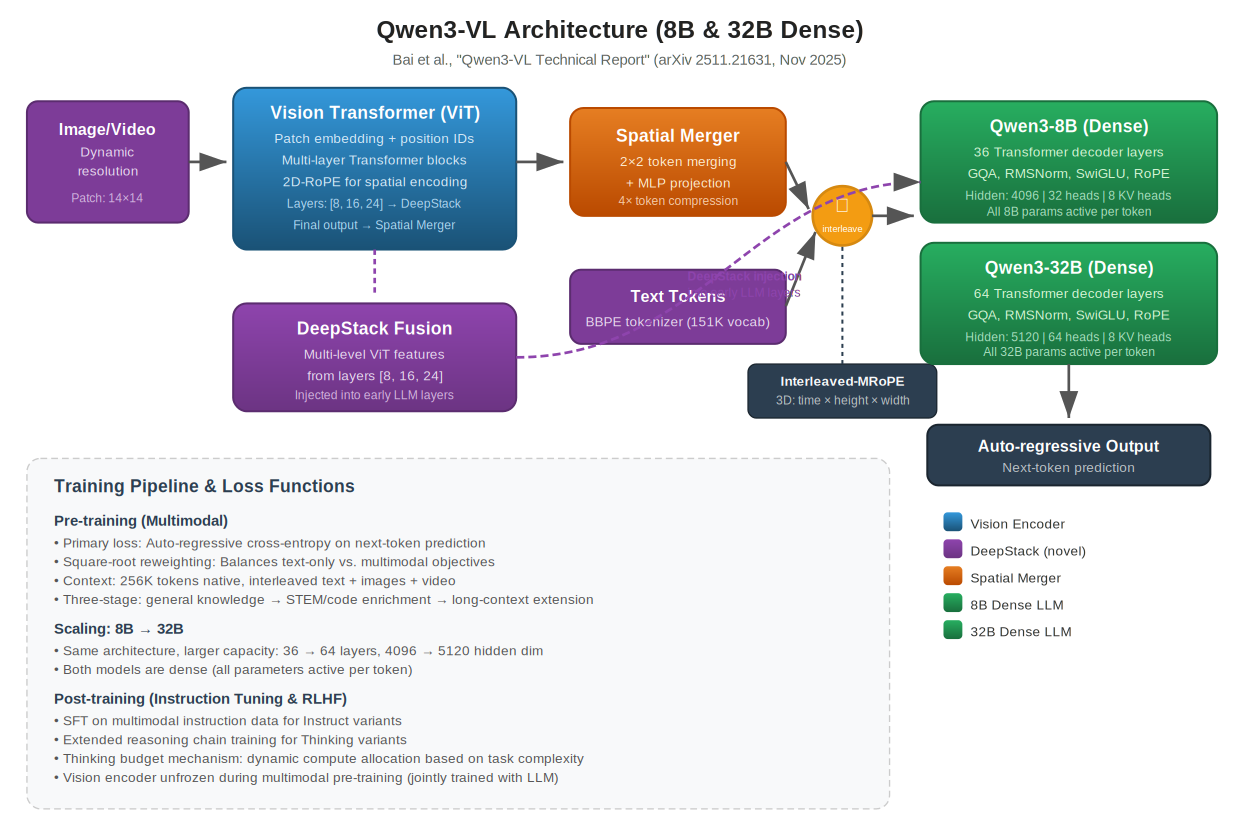
\includegraphics[width=0.95\textwidth]{figures/qwen3vl_architecture.png}
\caption{Qwen3-VL architecture (8B and 32B dense): jointly-trained ViT with DeepStack $\rightarrow$ Spatial Merger $\rightarrow$ Qwen3 decoder with Interleaved-MRoPE.}
\label{fig:qwen-arch}
\end{figure}

\subsection{\points{1} Encoders}

\textbf{LLaVA-1.5-7B} uses CLIP ViT-L/14 at fixed $336{\times}336$ resolution (576 patches $\times$ 1024-d, penultimate layer features). The encoder is \textbf{completely frozen}---a pure cross-modal transfer approach where CLIP's web-scale contrastive features are projected into the LLM's space without adaptation. This limits scientific figure understanding to what CLIP learned from general image-text pairs, which may not support the fine-grained numerical extraction our task demands (e.g., distinguishing a bar at 84.6\% from 89\%).

\textbf{Qwen3-VL (8B and 32B)} uses a ViT with \textbf{dynamic resolution} (variable patch counts preserving native aspect ratio) and \textbf{2D-RoPE} encoding spatial position within the ViT. This encoder is \textbf{jointly trained} with the LLM---a co-learning approach where visual and linguistic representations co-adapt, directly addressing the transference challenge. Our dataset's visual heterogeneity (tables 44.3\%, plots 28.1\%, schematics 17.4\%) creates a \textbf{quantification} challenge \citep{Liang-foundations-2024}: each figure type encodes information differently, and our H4 results confirm this---tables are easiest for verdict accuracy (51.4\% avg at 8B) but hardest for feedback quality (6.4\% match), while schematics benefit most from visual context (+9.4pp verdict, +25.0pp feedback at 8B).

\textbf{Alternative: SigLIP} replaces CLIP's softmax contrastive loss with sigmoid-based binary classification, offering better-calibrated visual-text matching scores potentially useful for partial-correctness detection. All three models process text through their LLM's token embedding layer; Qwen3-VL's 151K-token BPE vocabulary provides finer-grained tokenization of scientific terminology than LLaVA's 32K vocabulary.

\subsection{\points{1} Decoders}

\textbf{LLaVA-1.5-7B} uses Vicuna-7B v1.5 (LLaMA-2 fine-tune; 32 layers, 4096-d, GQA, SwiGLU, 1D RoPE, ${\sim}$4K context). Visual tokens from the 2-layer MLP projector (GELU, 1024$\rightarrow$4096) are concatenated with text tokens before the first layer---a shallow alignment creating a large modality gap.

\textbf{Qwen3-VL-8B} uses a 36-layer Qwen3 decoder (4096-d, 32 attention heads, 8 KV heads via GQA) with \textbf{Interleaved-MRoPE} encoding three spatial-temporal dimensions (24-d temporal, 20-d height, 20-d width), enabling the decoder to ground spatial claims to specific figure regions. Its \textbf{DeepStack} mechanism \citep{ge2024deepstack} injects multi-level ViT features from layers 8, 16, and 24 into early LLM layers, creating multiple transference pathways that preserve low-level visual details (character shapes for OCR, edges for trend detection). The 256K context window accommodates full paper context.

\textbf{Qwen3-VL-32B} scales the same architecture to 64 layers with 5120-d hidden dimensions, 64 attention heads, and 8 KV heads (32.8B total parameters). Our scaling experiments confirm the larger decoder provides substantially greater cross-modal reasoning capacity: multimodal feedback match improved from 6\% to 20\% (LLM judge, $n{=}50$), schematics' visual context benefit doubled from +9.4pp to +18.8pp for verdict accuracy, and visual context began \emph{helping} conceptual error detection (+2.4pp) whereas at 8B it hurt all error types. The shared DeepStack and MRoPE mechanisms mean both Qwen3-VL models use the same multi-level fusion strategy, with the 32B's additional depth providing more layers for integrating transferred visual information.

Our finding that auto metrics (${\sim}$0.30 F1 across all scenarios at both scales) failed to capture the 2$\times$ difference in feedback quality revealed by human evaluation (multimodal 80\% vs.\ text\_only 40\% at 8B) demonstrates a \textbf{quantification} failure \citep{Liang-foundations-2024}: standard NLP metrics cannot quantify cross-modal reasoning quality, motivating our LLM-as-judge and manual evaluation approach.

\subsection{\points{1} Loss Functions}

\textbf{Primary: Auto-regressive cross-entropy.} All three models use $\mathcal{L} = -\sum_i \log P(t_i \mid V, t_1, \ldots, t_{i-1})$ over response tokens only. We do not modify this for our inference-only experiments.

\textbf{Auxiliary 1: CLIP Contrastive Loss (InfoNCE).} This symmetric contrastive loss shaped LLaVA's frozen encoder features via image-text matching. The resulting coarse-grained alignment may explain why visual input hurts verdict accuracy for factual errors ($-$21.2pp at 8B)---CLIP features support semantic matching but not the precise numerical extraction needed to verify specific claims. Factual errors require \emph{non-redundant cross-modal interaction} \citep{Liang-foundations-2024}: the correct value exists only in the visual modality, the claimed value only in text, and the model must extract and compare both precisely.

\textbf{Auxiliary 2: Square-Root Reweighting.} Qwen3-VL scales multimodal sample loss by $\sqrt{N_\text{text}/N_\text{multimodal}}$ during pre-training, preventing degradation on text understanding while learning visual grounding. Our results confirm this dual capability matters: visual context helps all error types for feedback quality (factual +21.2pp, conceptual +31.7pp, omission +33.3pp at 8B) even while hurting verdict accuracy.

\textbf{Auxiliary 3 (Proposed): Verdict-Classification Head.} For future fine-tuning on SPIQA+, we propose extracting the hidden state at the verdict token position and passing it through a lightweight 3-class classification head supervised with cross-entropy against ground-truth labels. This would provide direct supervisory signal for the detection task (H1) alongside the generative explanation loss.

% Architecture Summary Table
\begin{table}[t]
\centering
\caption{Architecture summary of the three models used for SPIQA+ inference.}
\label{tab:arch-summary}
\small
\begin{tabular}{@{}lccc@{}}
\toprule
\textbf{Component} & \textbf{LLaVA-1.5-7B} & \textbf{Qwen3-VL-8B} & \textbf{Qwen3-VL-32B} \\
\midrule
Vision Encoder & CLIP ViT-L/14 (frozen) & ViT + 2D-RoPE (joint) & ViT + 2D-RoPE (joint) \\
Cross-Modal Bridge & 2-layer MLP & Spatial Merger + DeepStack & Spatial Merger + DeepStack \\
LLM Backbone & Vicuna-7B (32L, 4096-d) & Qwen3-8B (36L, 4096-d) & Qwen3-32B (64L, 5120-d) \\
Attention & GQA (32h) & GQA (32h / 8kv) & GQA (64h / 8kv) \\
Position Encoding & 1D RoPE & Interleaved 3D MRoPE & Interleaved 3D MRoPE \\
Context Length & ${\sim}$4K tokens & 256K tokens & 256K tokens \\
Transference & Cross-modal (frozen) & Co-learning (joint) & Co-learning (joint) \\
Loss Functions & AR cross-entropy & AR CE + $\sqrt{}$ reweight & AR CE + $\sqrt{}$ reweight \\
\bottomrule
\end{tabular}
\end{table}


\clearpage
\subsection{Team member contributions to this report}

\paragraph{Dipti Aswath} constructed 9 of the 18 ICL exemplars for SPIQA+ and led dataset validation (Phase 3: human spot-check of ${\sim}$20 examples, error distribution analysis, quality gate enforcement at $\geq$90\% agreement). Ran all H3 (error type) and H4 (figure type) experiments with the baseline model (Qwen3-VL-8B, $N{=}174$), producing both verdict accuracy and feedback quality results. Designed the hypothesis testing framework, performed cross-hypothesis analysis and synthesis (including the verdict--feedback dissociation finding and condition-routing proposal), and wrote Report 2.

\paragraph{Buddhika Makehelwala} led SPIQA+ dataset generation (Phase 2: GPT-5.1 synthetic generation of incorrect and partially correct student answers using the 18 ICL exemplars, producing the 174-example dataset). Selected the competitive model (Qwen3-VL-32B) and ran all competitive model experiments: H1/H2 ($N{=}50$) and H3/H4 ($N{=}174$) across all four conditions.

\paragraph{Jiashan Cui} developed and ran the evaluation pipeline for H1/H2 with the baseline model (Qwen3-VL-8B): automated metrics (F1, ROUGE-L, BLEU), LLM-as-Judge evaluation (Claude Sonnet 4), and human annotation ($n{=}10$ per condition). Extended evaluation to the competitive model (Qwen3-VL-32B) for H1/H2 with human evaluation and LLM-as-Judge, and ran human evaluation for H3/H4 competitive model results.

\paragraph{Khubi Shah} researched and identified Qwen3-VL models as competitive baselines for the project. Prepared the prompt structure used for inference across all conditions. Ran the baseline model (Qwen3-VL-8B) for H1/H2 across all four conditions ($N{=}50$). Authored the model proposal components: Encoders (Section 3.2), Decoders (Section 3.3), and Loss Functions (Section 3.4).


\nocite{*}
\bibliography{references}
\bibliographystyle{iclr2024_conference}

\appendix
\section{Appendix}

\subsection{Hypothesis Testing Summary}

We tested four hypotheses across two model scales (Qwen3-VL-8B and Qwen3-VL-32B). Table~\ref{tab:hypotheses} summarizes outcomes---note that most predictions failed, revealing unexpected patterns that inform the condition-routing key insight in Results.

\begin{table}[h]
\centering
\small
\begin{tabular}{@{}llll@{}}
\toprule
Hypothesis & Prediction & Verdict Result & Feedback Result \\
\midrule
H1: Multimodal Advantage & Visual input helps & FAIL ($-$8pp at 8B, $-$2pp at 32B) & PASS ($+$16pp soft match, 8B) \\
H2: Metric Alignment & Verdict $\propto$ feedback & FAIL (inversely correlated) & LLM Judge + Human validate \\
H3: Error Type & Factual $>$ Conceptual & FAIL (28.4\% $<$ 57.3\% at 32B) & Context helps conceptual more \\
H4: Figure Type & Tables $>$ Schematics & MIXED (32B: 51.1\% $<$ 57.0\%) & Schematics best at both scales \\
\bottomrule
\end{tabular}
\caption{Hypothesis results summary across both model scales.}
\label{tab:hypotheses}
\end{table}

\subsection{Error Type Analysis (H3 Detail)}

These tables break down H3 results by condition (C1--C4) for each error type. The $\Delta$ column shows multimodal benefit (C4$-$C1).

\vspace{4pt}
\noindent\textbf{Key patterns in Table~\ref{tab:h3_verdict} (Verdict):}
\begin{itemize}[itemsep=1pt, topsep=2pt, leftmargin=*]
  \item Factual errors are hardest (28--39\% avg)---visual context \textit{hurts} at both scales
  \item Conceptual errors are easiest (54--57\% avg)---32B C4 is the \textit{only} positive $\Delta$
  \item Omission errors hurt most by visual context at 32B ($-$26.7pp)
\end{itemize}

\begin{table}[h]
\centering
\small
\begin{tabular}{@{}llrrrrrr@{}}
\toprule
Model & Error Type & C1 & C2 & C3 & C4 & Avg & $\Delta$ (C4$-$C1) \\
\midrule
\multirow{3}{*}{8B} & Factual ($n{=}52$) & 51.9\% & 40.4\% & 34.6\% & 30.8\% & 39.4\% & $-$21.2pp \\
 & Conceptual ($n{=}41$) & 63.4\% & 61.0\% & 43.9\% & 48.8\% & 54.3\% & $-$14.6pp \\
 & Omission ($n{=}15$) & 53.3\% & 33.3\% & 46.7\% & 46.7\% & 45.0\% & $-$6.7pp \\
\midrule
\multirow{3}{*}{32B} & Factual ($n{=}52$) & 32.7\% & 28.8\% & 26.9\% & 25.0\% & 28.4\% & $-$7.7pp \\
 & Conceptual ($n{=}41$) & 58.5\% & 56.1\% & 53.7\% & 61.0\% & 57.3\% & \textbf{+2.4pp} \\
 & Omission ($n{=}15$) & 66.7\% & 53.3\% & 33.3\% & 40.0\% & 48.3\% & $-$26.7pp \\
\bottomrule
\end{tabular}
\caption{Verdict accuracy by error type and condition. Conceptual at 32B C4 is the \textit{only} cell where visual context improves verdict accuracy.}
\label{tab:h3_verdict}
\end{table}

\noindent\textbf{Key patterns in Table~\ref{tab:h3_feedback} (Feedback):}
\begin{itemize}[itemsep=1pt, topsep=2pt, leftmargin=*]
  \item \textit{All} error types benefit from visual context ($+$21--33pp)---opposite of verdict
  \item Conceptual errors have highest feedback quality (42--43\% avg)
  \item Omission errors show largest gains but remain hardest (13--15\% avg)
\end{itemize}

\begin{table}[h]
\centering
\small
\begin{tabular}{@{}llrrrrrr@{}}
\toprule
Model & Error Type & C1 & C2 & C3 & C4 & Avg & $\Delta$ (C4$-$C1) \\
\midrule
\multirow{3}{*}{8B} & Factual & 13.5\% & 25.0\% & 28.8\% & 34.6\% & 25.5\% & +21.2pp \\
 & Conceptual & 26.8\% & 51.2\% & 36.6\% & 58.5\% & 43.3\% & +31.7pp \\
 & Omission & 0.0\% & 0.0\% & 26.7\% & 33.3\% & 15.0\% & +33.3pp \\
\midrule
\multirow{3}{*}{32B} & Factual & 13.5\% & 26.9\% & 28.8\% & 34.6\% & 26.0\% & +21.2pp \\
 & Conceptual & 26.8\% & 48.8\% & 36.6\% & 56.1\% & 42.1\% & +29.3pp \\
 & Omission & 0.0\% & 0.0\% & 26.7\% & 26.7\% & 13.4\% & +26.7pp \\
\bottomrule
\end{tabular}
\caption{Feedback match rate (LLM-as-Judge) by error type and condition. Visual context helps feedback quality for \textit{all} error types at both scales ($+$21--33pp).}
\label{tab:h3_feedback}
\end{table}

\subsection{Figure Type Analysis (H4 Detail)}

These tables break down H4 results by condition (C1--C4) for each figure type. The $\Delta$ column shows multimodal benefit (C4$-$C1).

\vspace{4pt}
\noindent\textbf{Key patterns in Table~\ref{tab:h4_verdict} (Verdict):}
\begin{itemize}[itemsep=1pt, topsep=2pt, leftmargin=*]
  \item Schematics benefit most from visual context ($+$9.4pp at 8B, $+$18.8pp at 32B)
  \item Plots are consistently hurt by visual context ($-$10.3pp at 8B, $-$4.4pp at 32B)
  \item Tables show minimal change across conditions (51\% avg at both scales)
\end{itemize}

\begin{table}[h]
\centering
\small
\begin{tabular}{@{}llrrrrrr@{}}
\toprule
Model & Figure Type & C1 & C2 & C3 & C4 & Avg & $\Delta$ (C4$-$C1) \\
\midrule
\multirow{3}{*}{8B} & Table ($n{=}70$) & 52.9\% & 51.4\% & 51.4\% & 50.0\% & 51.4\% & $-$2.9pp \\
 & Plot ($n{=}68$) & 55.9\% & 47.1\% & 42.6\% & 45.6\% & 47.8\% & $-$10.3pp \\
 & Schematic ($n{=}32$) & 50.0\% & 46.9\% & 37.5\% & 59.4\% & 48.4\% & \textbf{+9.4pp} \\
\midrule
\multirow{3}{*}{32B} & Table ($n{=}70$) & 51.4\% & 51.4\% & 48.6\% & 52.9\% & 51.1\% & +1.4pp \\
 & Plot ($n{=}68$) & 52.9\% & 47.1\% & 48.5\% & 48.5\% & 49.3\% & $-$4.4pp \\
 & Schematic ($n{=}32$) & 46.9\% & 56.2\% & 59.4\% & 65.6\% & \textbf{57.0\%} & \textbf{+18.8pp} \\
\bottomrule
\end{tabular}
\caption{Verdict accuracy by figure type and condition ($N{=}174$). Schematics benefit most from visual context at both scales; plots are consistently hurt.}
\label{tab:h4_verdict}
\end{table}

\noindent\textbf{Key patterns in Table~\ref{tab:h4_feedback} (Feedback):}
\begin{itemize}[itemsep=1pt, topsep=2pt, leftmargin=*]
  \item \textit{All} figure types benefit from visual context ($+$7--34pp)---opposite of verdict for plots
  \item Schematics achieve highest feedback quality (35--46\% avg)
  \item Tables are hardest for feedback (6--12\% avg) despite being easiest for verdict
\end{itemize}

\begin{table}[h]
\centering
\small
\begin{tabular}{@{}llrrrrrr@{}}
\toprule
Model & Figure Type & C1 & C2 & C3 & C4 & Avg & $\Delta$ (C4$-$C1) \\
\midrule
\multirow{3}{*}{8B} & Table ($n{=}70$) & 1.4\% & 4.3\% & 11.4\% & 8.6\% & 6.4\% & +7.1pp \\
 & Plot ($n{=}68$) & 13.2\% & 25.0\% & 16.2\% & 32.4\% & 21.7\% & +19.1pp \\
 & Schematic ($n{=}32$) & 25.0\% & 37.5\% & 28.1\% & 50.0\% & \textbf{35.2\%} & +25.0pp \\
\midrule
\multirow{3}{*}{32B} & Table ($n{=}70$) & 4.3\% & 7.1\% & 17.1\% & 20.0\% & 12.1\% & +15.7pp \\
 & Plot ($n{=}68$) & 10.3\% & 32.4\% & 19.1\% & 44.1\% & 26.5\% & +33.8pp \\
 & Schematic ($n{=}32$) & 31.2\% & 50.0\% & 46.9\% & 56.2\% & \textbf{46.1\%} & +25.0pp \\
\bottomrule
\end{tabular}
\caption{Feedback match rate (LLM-as-Judge) by figure type and condition. Schematics achieve the highest feedback quality at both scales; tables are worst. Visual context helps feedback for \textit{all} figure types at both scales.}
\label{tab:h4_feedback}
\end{table}

\subsection{8B $\rightarrow$ 32B Scaling Comparison}

\noindent\textbf{Key improvements at 32B:}
\begin{itemize}[itemsep=1pt, topsep=2pt, leftmargin=*]
  \item Multimodal feedback quality jumps from 6\% to 20\% match ($+$14pp)
  \item Schematics: visual context benefit doubles for verdict ($+$18.8pp vs $+$9.4pp at 8B)
  \item Conceptual errors: visual context now \textit{helps} verdict ($+$2.4pp vs $-$14.6pp at 8B)
  \item Plot feedback: context benefit nearly doubles ($+$33.8pp vs $+$19.1pp)
\end{itemize}

\noindent\textbf{Still challenging at 32B:}
\begin{itemize}[itemsep=1pt, topsep=2pt, leftmargin=*]
  \item Factual errors remain hard (28.4\% avg) with visual context still hurting verdict ($-$7.7pp)
  \item Text-only feedback quality unchanged (2\% match at both scales)
  \item Plots still hurt by visual context for verdict ($-$4.4pp)
  \item Omission errors: visual context hurts verdict \textit{more} at 32B ($-$26.7pp vs $-$6.7pp at 8B)
\end{itemize}

\subsection{Auto Metrics vs.\ LLM-as-Judge}

Traditional auto metrics (F1, ROUGE-L, BLEU) fail to differentiate feedback quality across conditions, motivating our use of LLM-as-Judge evaluation:

\begin{table}[h]
\centering
\small
\begin{tabular}{@{}lrrr@{}}
\toprule
Metric & 8B Range & 32B Range & Differentiates? \\
\midrule
F1 & 0.29 -- 0.30 & 0.294 -- 0.325 & No \\
ROUGE-L & 0.18 -- 0.20 & 0.192 -- 0.207 & No \\
BLEU & 4.8 -- 6.7 & 5.93 -- 8.13 & No \\
LLM Judge (Soft Match) & 40\% -- 56\% & 42\% -- 58\% & Yes \\
Human Eval (Match) & 40\% -- 80\% & - & Yes \\
\bottomrule
\end{tabular}
\caption{Evaluation method comparison. Only LLM-as-Judge and human evaluation differentiate feedback quality across conditions.}
\label{tab:auto_metrics}
\end{table}

\subsection{Statistical Notes}

\begin{itemize}[itemsep=1pt, topsep=2pt, leftmargin=*]
  \item \textbf{H1/H2 sample size:} $n{=}50$ yields ${\sim}$7pp confidence intervals; differences $<$5pp are noise
  \item \textbf{Borderline significance:} The 8pp gap (text-only 56\% vs multimodal 48\%) at 8B is at the edge of significance
  \item \textbf{Human evaluation:} $n{=}10$ per condition means each example shifts match rate by 10pp
  \item \textbf{H3/H4 reliability:} Full $N{=}174$ sample provides tighter confidence intervals (${\sim}$4--5pp)
\end{itemize}

\subsection{Next Steps}

\noindent\textbf{Priority actions for future work:}
\begin{enumerate}[itemsep=1pt, topsep=2pt, leftmargin=*]
  \item \textbf{Chain-of-thought prompting:} Force explicit figure description before judgment---targets factual errors and plot interpretation
  \item \textbf{Larger model scale:} Test Qwen3-VL-235B-A22B (MoE, 22B active)---may extend scaling gains to factual errors
  \item \textbf{Larger evaluation samples:} 200+ examples to shrink confidence intervals from ${\sim}$7pp to ${\sim}$3--4pp
  \item \textbf{C5 condition:} Add multimodal + paper paragraphs for conceptual/omission errors requiring experimental context
\end{enumerate}

\end{document}
